System tests consist of 14 maps of different sizes and complexity levels. Each algorithm is tested with every map with the same positioning of the agents. Test time is defined as end end-to-end time, starting from test triggering alculation by te agent  and stopping when the the path is ready. More detailed information such as "test setup time", "communication time" and "algorithm calculation time" can be found in the observability suite(grafana).

\subsection{System simulated in the cloud}
This system can be simulated both in a local environment as well as in the cloud. Multiple agents can be created and connected to a system by spawning multiple Kubernetes pods. This scenario is not taking into account communication delay as all containers are communicating in a local network(cluster network).

\subsection{Real system}
A small system composed of three external devices(raspberry pi) was created to showcase how a real system would work. In each of the devices, an agent container was deployed. On one of them, there are map-servcie and broker containers. The scheme of the device's connection can be seen in diagram \ref{fig:cluster}.
\begin{figure}[H]
    \centering
    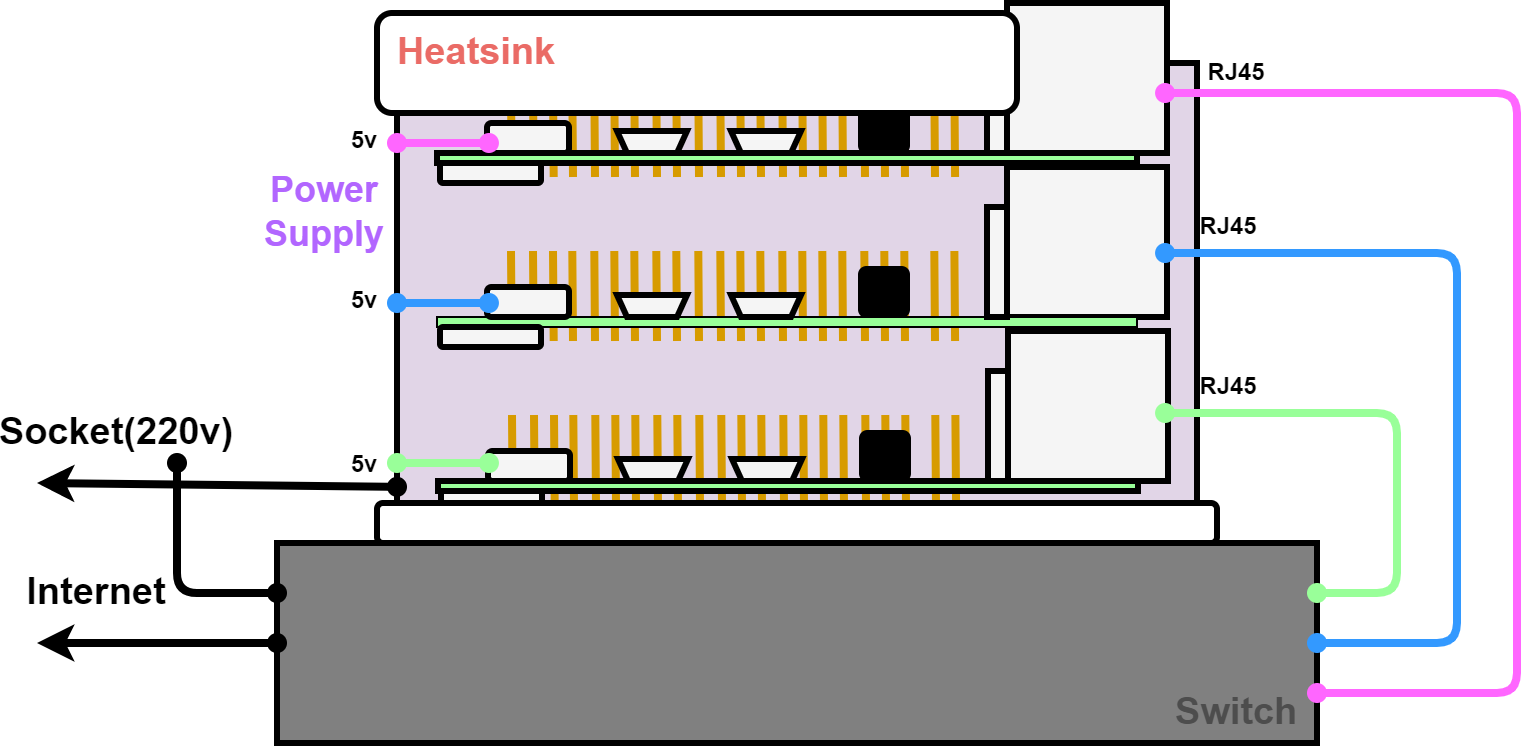
\includegraphics[width=0.8\textwidth]{pictures/cluster.png}
    \caption{ Real cluster }
    \label{fig:cluster}
\end{figure}

This setup resembles a real-world scenario, with 3 robots(agents) and one server meant for deploying brokers and communicating to the cloud. Agents have limited resources as Single Board Computer used for deployment only has 1GB of memory and Quad-core Cortex-A72 1.5GHz processor\cite{rpi_specs}. For the purpose of the test, computing power can also be throttled. Devices are connected to the local network via an internet switch. 

The challenging part was that those devices are using ARM architecture, therefore containers have to be rebuilt to support this architecture. To ease a development struggle, azure DevOps agents were installed on the machines and a Continous Integration pipeline was put in place, which rebuilds ARM images on every code change using local machines as hosts and pushes them into the image registry. The cloud part of the solution is deployed in okteto cloud and both parts are exchanging messages via MQTT brokers.

\subsection{System composed from virtual machines}
Another way of testing the system is to create a set of virtual machines or containers locally and connect them to the cloud system. The benefits of this approach are that this setup is easier to maintain, supports x86 architecture, and is easily extensible, as for spawning more agents there is no additional hardware needed. Resource limits can also be implemented both in the case of containers and virtual machines. Those entities have to be put in the same virtual network to enable communication between simulated machines.